\documentclass[11pt,a4paper]{article}

\usepackage[utf8]{inputenc}
\usepackage{times}
\usepackage[left=2cm,top=3cm,text={17cm, 24cm}]{geometry}
\usepackage[czech]{babel}
\usepackage{graphicx}
\usepackage{setspace}
\usepackage{hyperref}
\usepackage{multirow}
\usepackage{pdflscape}
\usepackage{url}
\DeclareUrlCommand\urlmoje{\urlstyle{tt}}
\bibliographystyle{czplain}

\begin{document}

    \begin{titlepage}
    \begin{center}
      {\Huge
      \textsc{Vysoké učení technické v~Brně} \\
      \medskip
		\huge{\textsc{Fakulta informačních technologií}}
       }\\
      %\vspace{\stretch{0.191}}
      \begin{figure}[h]
		\begin{center}
		\scalebox{0.8}{
\includegraphics{fit.png}}
		\end{center}
	  \end{figure}
	  %\vspace{\stretch{0.191}}
      {\LARGE
      Dokumentace k projektu do předmětů IFJ a IAL}\\
      \LARGE{\textbf{Implementace překladače imperativního jazyka IFJ17}}
      \vspace{\stretch{0.060}}

      {\LARGE Tým 065, varianta I}

      {\LARGE 31. března 2017}
      \vspace{\stretch{0.618}}

      {\LARGE Seznam autorů:\\}
      {\Large\itshape Vedoucí: Bártl Roman (xbartl06) - 25\%\par}
        {\Large\itshape Bartošek Jan (xbarto92) - 25\%\par}
        {\Large\itshape Odehnal Tomáš (xodehn08) - 25\%\par}
        {\Large\itshape Šopf Petr (xsopfp00) - 25\%\par}
        \vspace{\stretch{0.718}}
        {\Large \textbf{Rozšíření:} UNARY, BASE, IFTHEN}
        \vspace{\stretch{0.2}}
    \end{center}
\end{titlepage}

    \doublespacing
	\tableofcontents
	\singlespacing
    \newpage

\addtocontents{toc}{\setcounter{tocdepth}{3}}
\section{Scanner}
Implementoval xbarto92

	\subsection{Postup implementace}
	Při prvním návrhu lexikální analýzy jsem se inspiroval ukázkovým příkladem, kde byl scanner řešený s využitím přepínače switch umístěného v nekonečné smyčce. První verze scanneru spatřila světlo světa již 7. října, ovšem její funkčnost byla naprosto nevyhovující, a tak jsem scanner postupně opravoval a rozšiřoval.

	Původní verze scanneru vracela pouze hodnotu datového typu integer, která reprezentovala přečtený lexém a nedokázala rozlišovat klíčová slova od identifikátorů. Tento problém jsem vyřešil vytvořením pole, jehož hodnoty odpovídají všem rezervovaným klíčovým slovům a v případě zjištění identifikátoru, pak jeho porovnáním.

	Následovalo vytvoření struktury reprezentující token nesoucí informace o typu přečteného lexému (číslo, ID, atd..), jeho hodnotu (např.: název proměnné) a v poslední řadě zde byla přidána i hodnota řádku, která slouží pro výpis chybových hlášek a lepší debug. Dřívější myšlenka byla taková, že scanner by měl hodnotu přečteného tokenu hned zapsat do tabulky symbolů. Z tohoto důvodu jsem připravil binární strom a dynamický stack, právě pro práci s touto tabulkou. Nicméně po delší úvaze jsme se rozhodli zanechat tuto úlohu mimo parser, a tak se jejím vyřešením zaobírali mí kolegové.

	V momentě, kdy scanner již obstojně interpretoval jakýkoliv příchozí lexém jsem se začal zaobírat rozšířeními UNARY a BASE, kde první z nich jsem jako speciální token posílal ke zpracování parseru, a ten druhý nahrál a funkcí \emph{strtol()} převedl hodnotu čísla do dekadické soustavy a posílal jako jakékoli jiné číslo. V neposlední řadě jsem se zaobíral testováním všech možných chybových stavů a jejich správným řešením.

	\subsection{Funkce}
	Lexikální analýza implementovaná v souborech \emph{scanner.c} a \emph{scanner.h} cyklicky načítá ze vstupu znak po znaku a každý ihned interpretuje a kontroluje jejich vzájemnou návaznost.

	Funkce getNextToken(), která obstarává celou lexikální analýzu, se volá v parseru při potřebě následujícího tokenu. Při správné posloupnosti znaků je vrácen token, neboli struktura, která se skládá ze tří hodnot (viz výše). V opačném případě se na chybový výstup vypíše odpovídající chybová hláška spolu s řádkem v kódu, na kterém k chybě došlo.
    \newpage

\subsection{Konečný Automat Lexikální Analýzy}
    \vspace{1cm}

    \begin{figure}[h!]
        \centering
        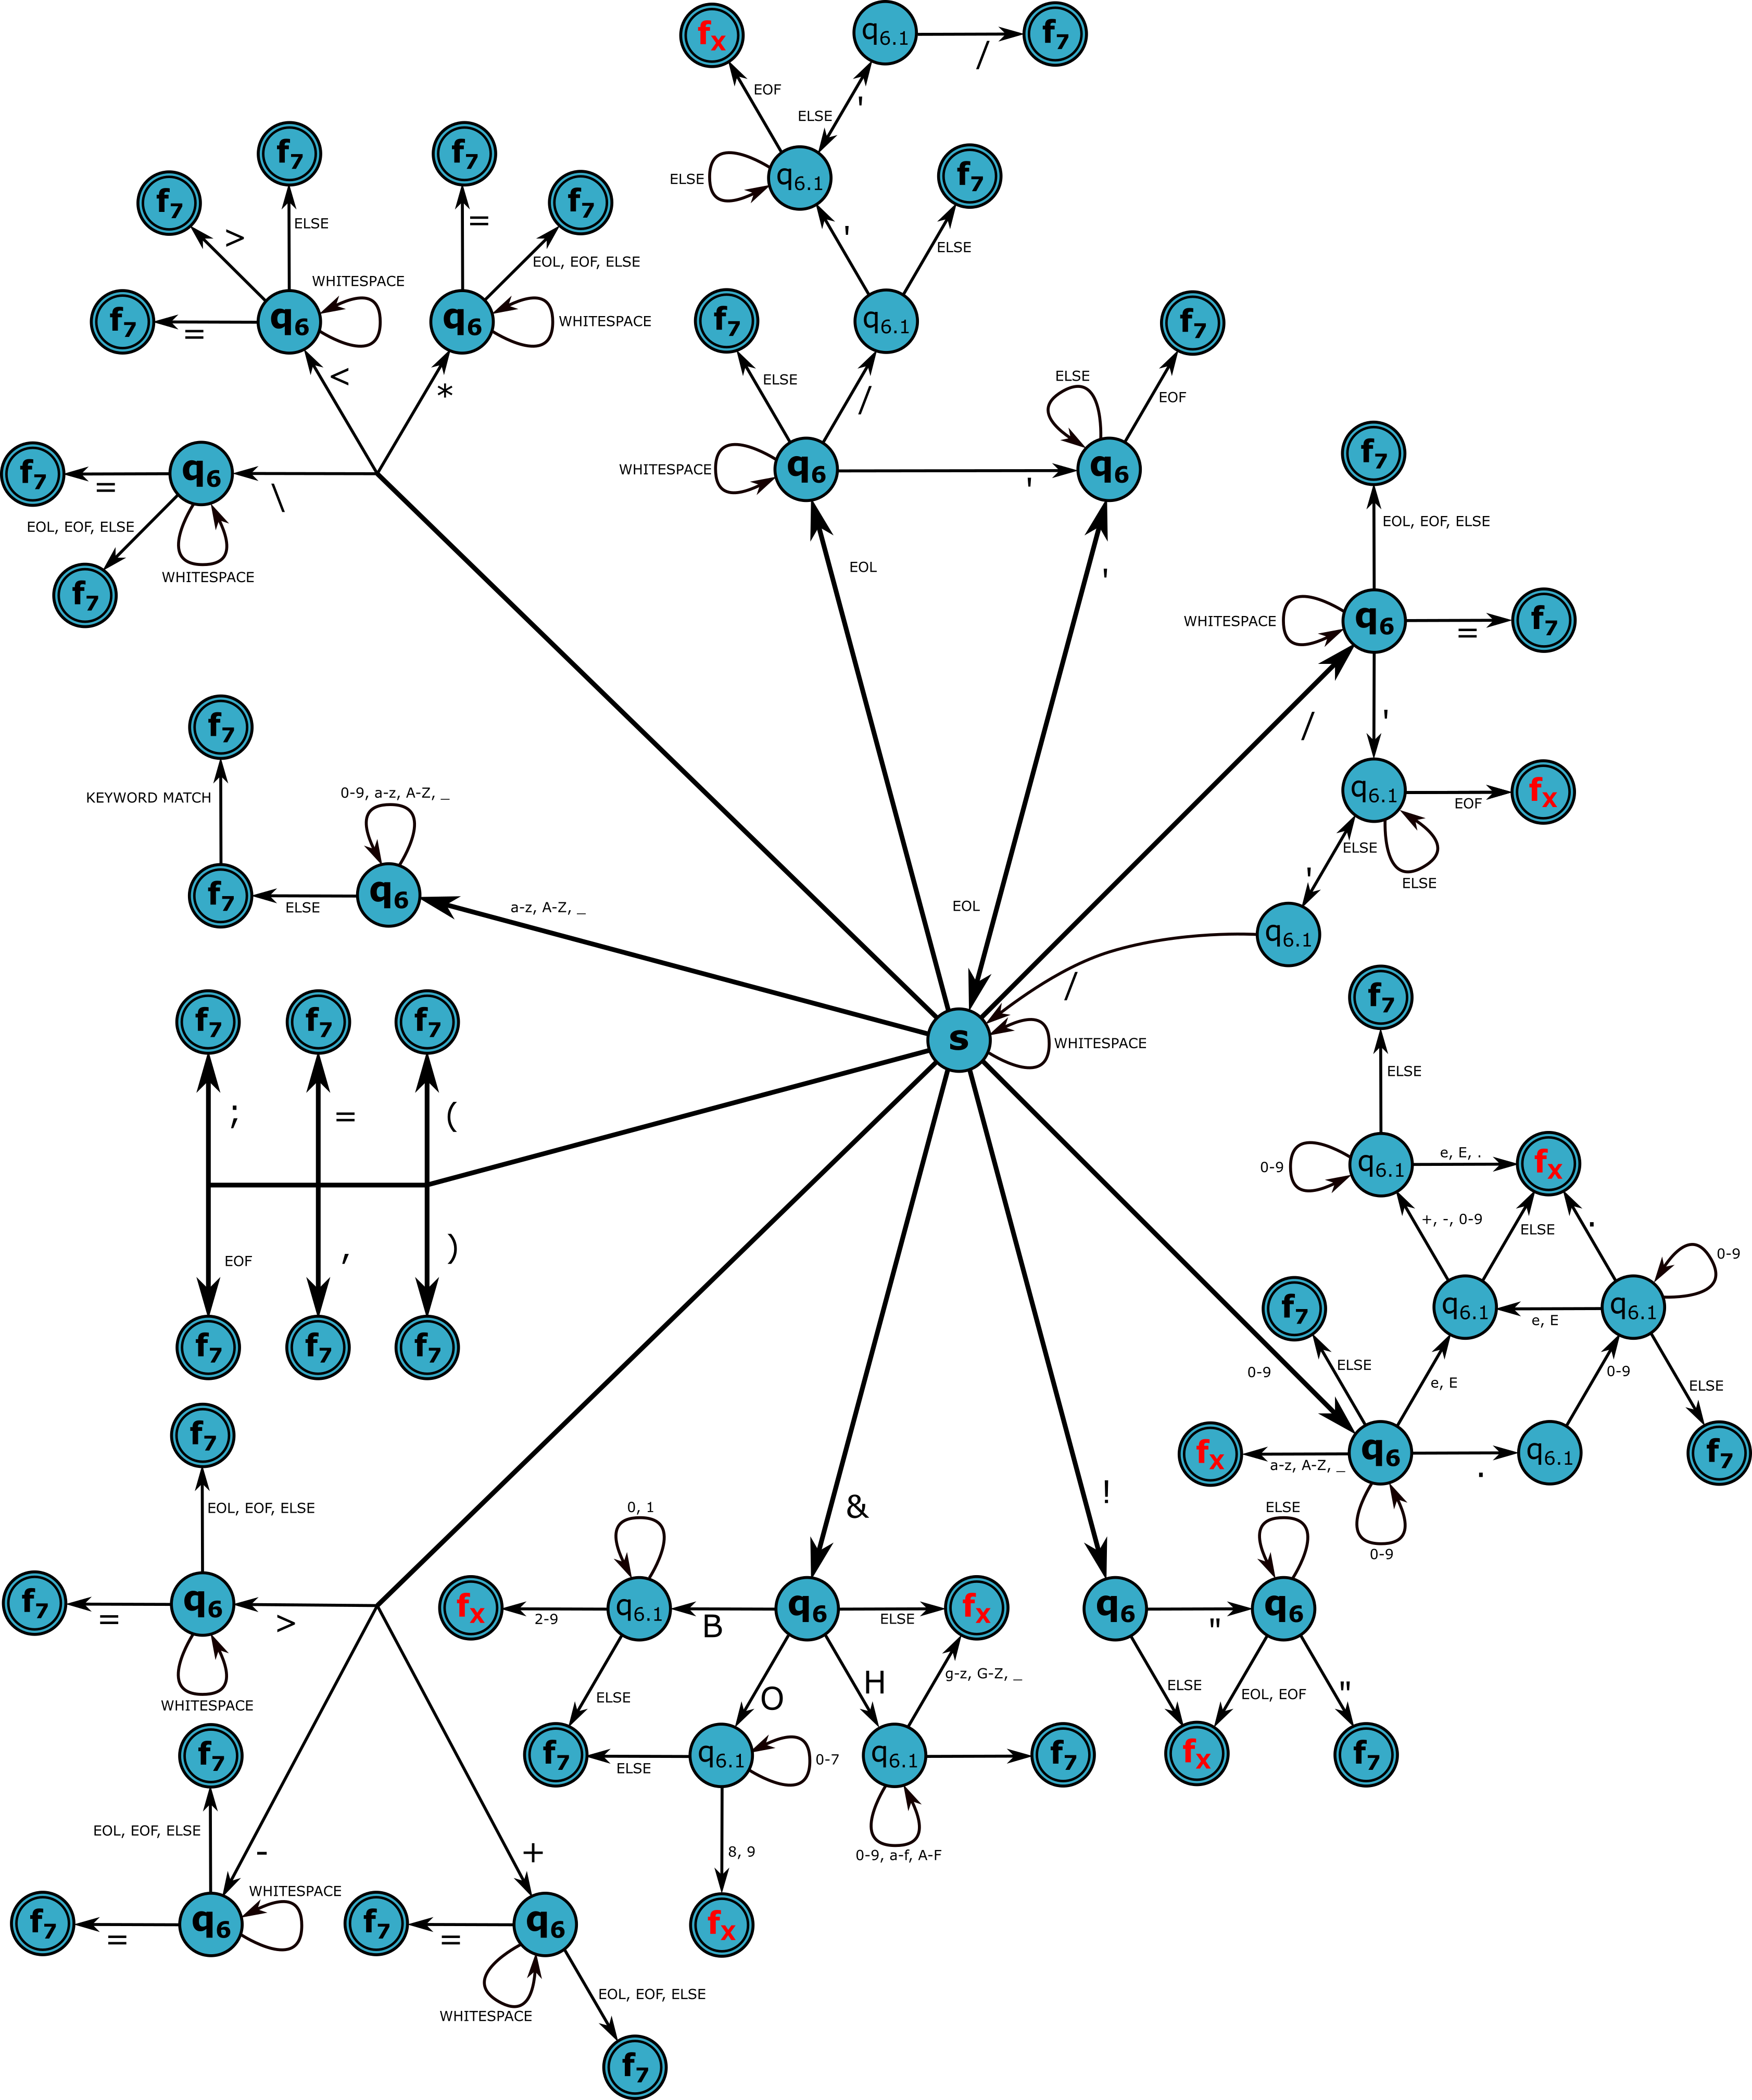
\includegraphics[height=20cm]{KA.png}
        \caption{Konečný automat lexikální analýzy}
        \label{obr:LA}
    \end{figure}

	\newpage


\section{Parser - Syntax}
    Implementoval xbartl06

    \subsection{Funkce}
    Syntaktická analýza (dále jen SA) má za úkol simulovat činnost derivačního stromu podle pravidel LL-gramatiky daného jazyka a kontrolovat jeho správné zapsání z hlediska syntaxe. Dále využívá precedenční tabulky pro analýzu zdola-nahoru pro zpracování výrazů. Parser je rozšířen o sémantickou analýzu (více o sémantice v kapitole \ref{semantika}).


    \subsection{Postup implementace}
    Před samotnou implementací SA bylo zapotřebí sestavit LL-gramatiku určující pravidla jazyka IFJ17 (viz obázek \ref{obr:LLG}), k LL-gramatice i LL-tabulku (viz obrázky \ref{obr:LLT1} a \ref{obr:LLT2}) a precedenční tabulku pro zpracovávání výrazů (viz obrázek \ref{obr:PT}).

    Po návrhu všech těchto částí jsem mohl začít se samotnou implementací parseru. Pro konstrukci SA jsme se dohodli, že využijeme doporučenou metodu rekurzivního sestupu. Vstupem pro SA je sekvence tokenů, které vytváří a posílá lexikální analyzátor. Na základě informací obsažených v těchto tokenech a pravidel LL-gramatiky se dá určit, zda-li je vstupní kód syntakticky správně či nikoliv.

    Jednotlivé funkce představují neterminály, které postupně kontrolují, zda jsou všechny terminály ve formě tokenů ve správném pořadí (syntakticky správně). V opačném případě vrací chybovou hlášku s patřičným chybovým kódem. Precedenční tabulku pro zpracování výrazů jsem upravil tak, abych si co nejvíce usnadnil práci (více v kapitole \ref{Prec_Analyza}).


        \subsubsection{LL-gramatika} \label{LL_Gramatika}

        Následující obrázek \ref{obr:LLG} ukazuje řešení LL-gramatiky. Některá pravidla nemusejí být na první pohled dobře pochopitelná, proto se je pokusím co nejlépe vysvětlit.

        U pravidla 18 a 30 jsou terminály sepsány v množinách z důvodu, abych zkrátil zápis pravidel a neopakovalo se jedno a to samé pravidlo, které má rozdílný pouze první terminál. Také je více názorné, že se jedná o totéž pravidlo, a v samotné implementaci se pouze pomocí podmínky testuje, zda-li je právě zpracovávaný lexém, jedním z těchto terminálů. Dále u pravidla 31 nejsou unární přiřazení z toho důvodu, že jsme neimplementovali rozšíření FUNEXP, tudíž nemůže být volání funkce součástí výrazu.

        Dále jsem abstrahoval terminály \emph{End-Of-File} (dále jen \emph{EOL}) a \emph{End}, které jsou použity u vícero pravidel. Ačkoliv se to může zdát zbytečné, tak toto řešení opět naznačuje samotnou implementaci, kdy stačí zavolat funkci, která kontroluje, zda následuje lexém \emph{EOL} (respektive \emph{End}) a není již potřeba rozepisovat podmínky všude, kde by se měl nacházet tento lexém \emph{EOL} (respektive \emph{End}).

        Neterminál \emph{$<$expression$>$} značící výraz, již není v LL-gramatice rozepsán, protože se dále zpracovává pomocí precedenční SA (viz kapitola \ref{Prec_Analyza}).

        \newpage

            \begin{figure}[h!]
                \centering
                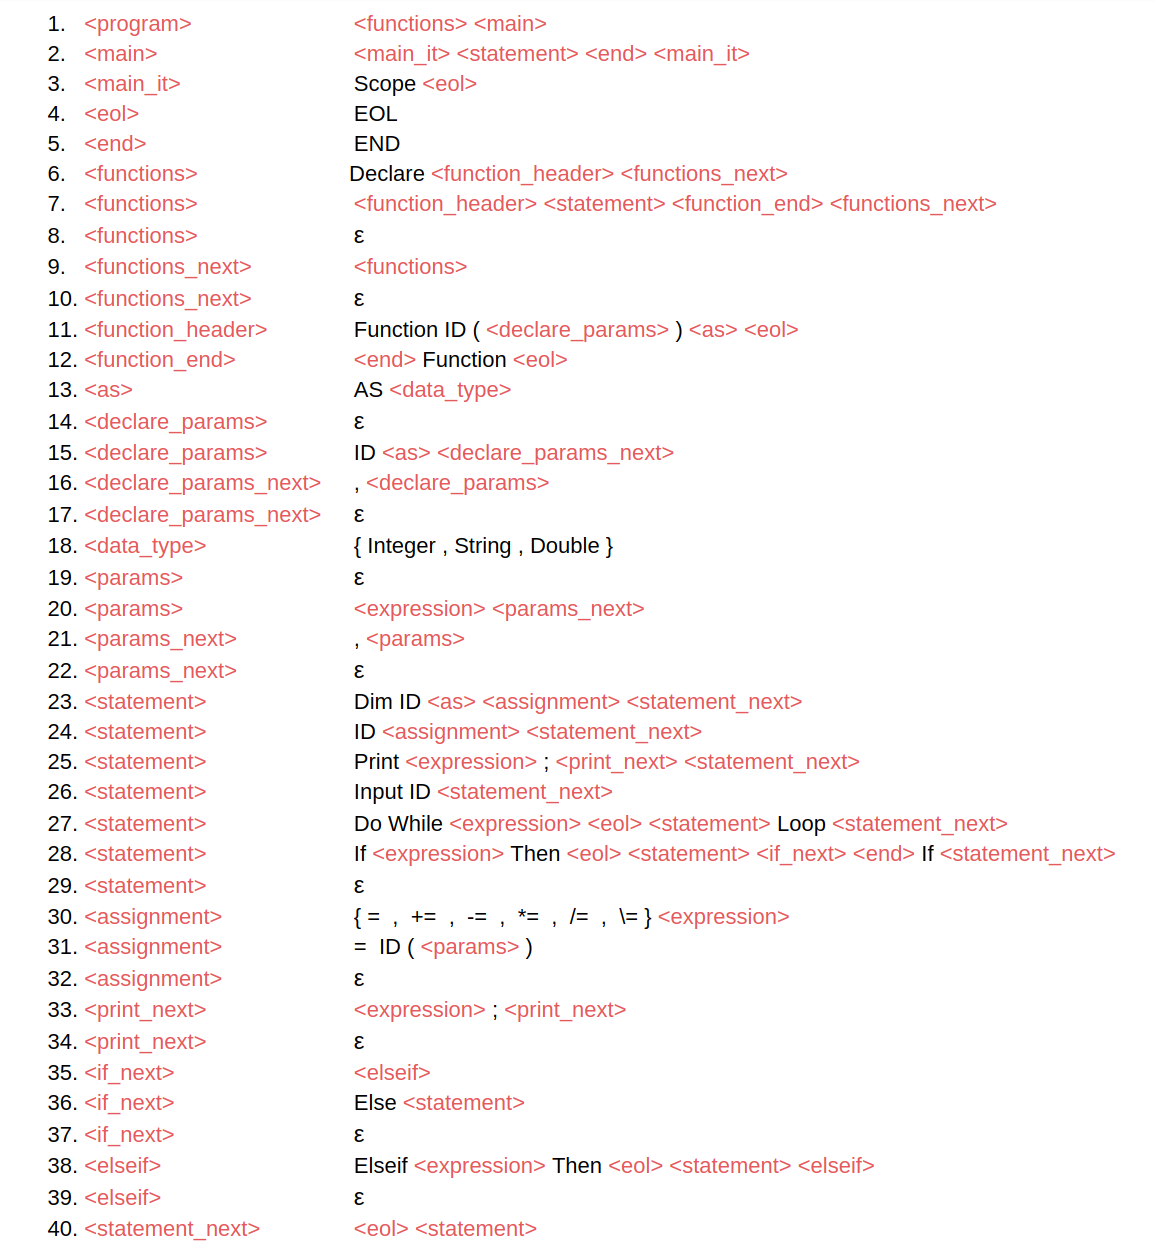
\includegraphics[width=17cm]{LLGram.png}
                \caption{LL-gramatika}
                \label{obr:LLG}
            \end{figure}

        \newpage

        \subsubsection{LL-tabulka} \label{LL_Tabulka}

            Na následujících dvou obrázcích je zobrazena LL-tabulka, kterou jsem z důvodu velikosti musel rozdělit na dvě části. Jednotlivá čísla v tabulce odkazují na pravdila LL-gramatiky (viz obrázek \ref{obr:LLG}). Dále jsem v tomto případě neterminál \emph{$<$expression$>$} zde uvedl jako terminál, jelikož není zpracováván SA shora-dolů.

            \vspace{1cm}

            \begin{figure}[h!]
                \centering
                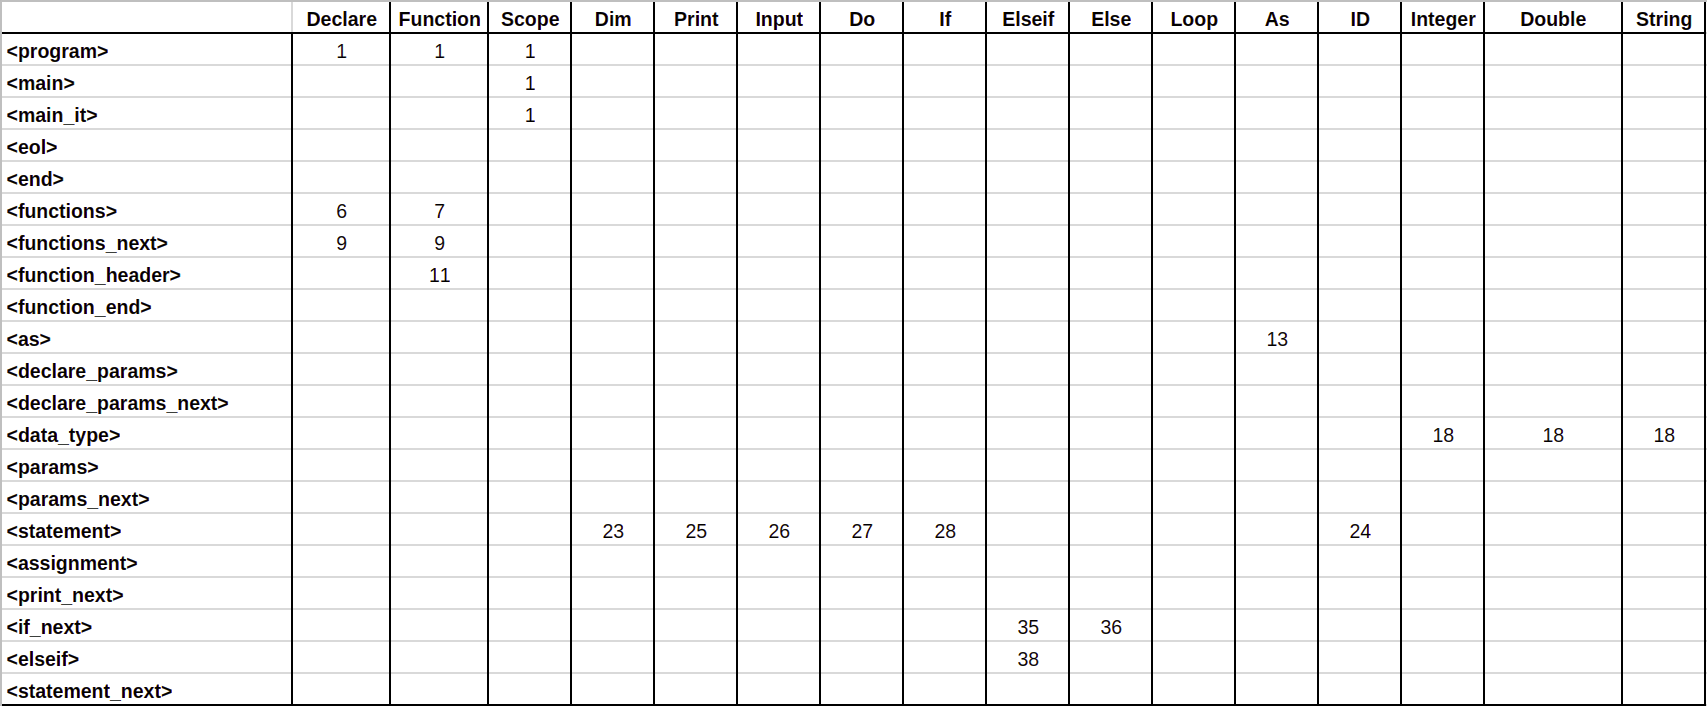
\includegraphics[width=17cm]{LLTable.png}
                \caption{LL-tabulka}
                \label{obr:LLT1}
            \end{figure}


            \begin{figure}[h!]
                \centering
                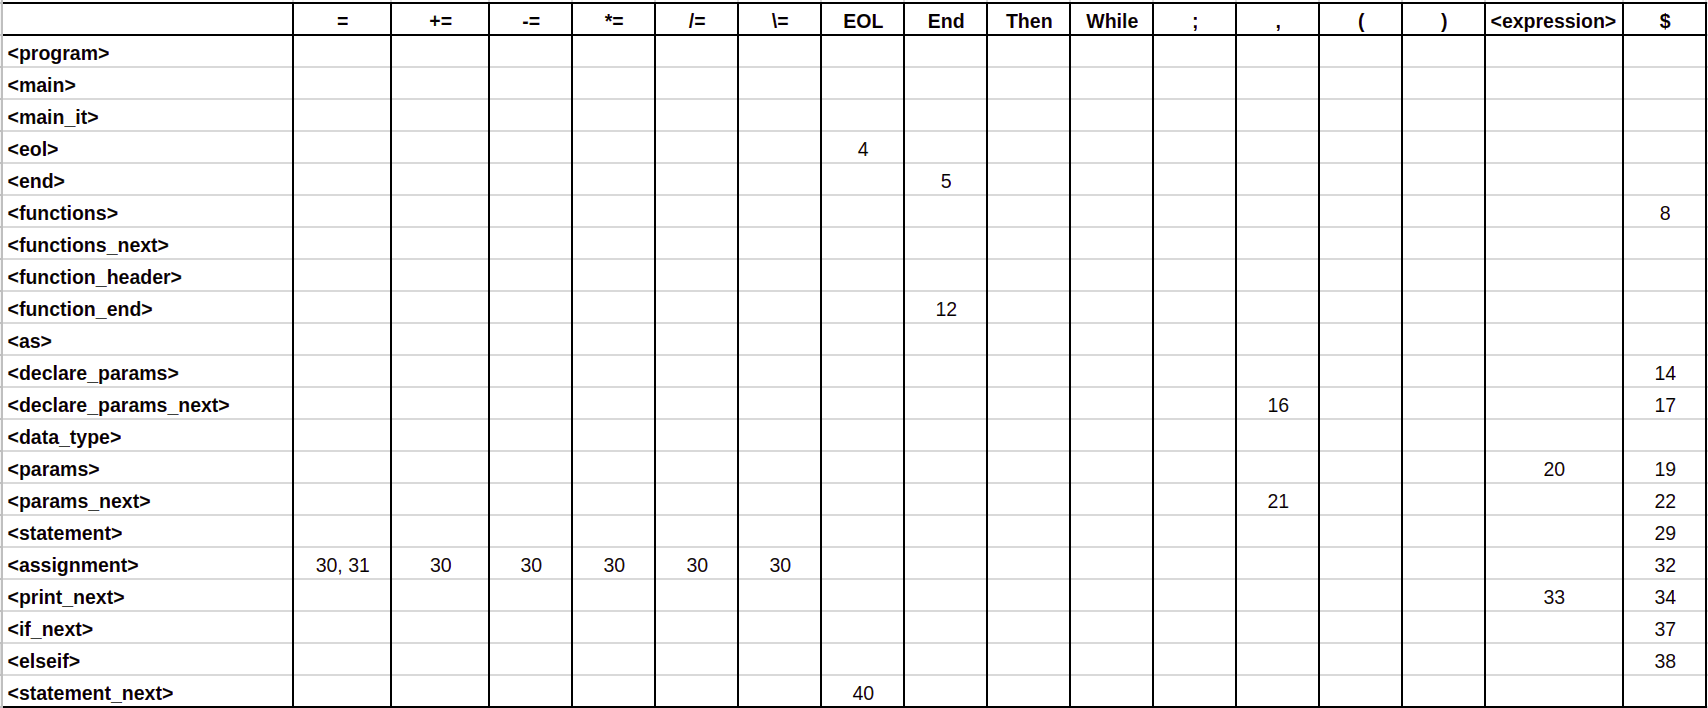
\includegraphics[width=17cm]{LLTable2.png}
                \caption{LL-tabulka - pokračování}
                \label{obr:LLT2}
            \end{figure}

        \newpage

        \subsubsection{Precedenční analýza} \label{Prec_Analyza}
        Precedenční SA, jak již bylo zmíněno výše, slouží ke zpracování výrazů. Kdykoliv se v parseru narazí na pravidlo, kde je očekávaný výraz, zavolá parser funkci pro jeho pracování, která se nachází v souboru \emph{precedence.c}.

        Pro precedenční analýzu je využit zásobník, do kterého se postupně zapisují jednotlivé terminály (čísla, proměnné, operátory, aj.) a neterminály výrazu ($E$ – zpracovaná část výrazu, $<$ - shift, $>$ - redukce). Samotná precedenční tabulka je uložna jako dvourozměrné pole kvůli jednoduchému vyhledávání v ní.

        Kromě běžných neterminálů jako $<$, $>$, $=$ a prázdné políčko (v našem případě označeno jako B) značící chybu, jsem tabulku rozšířil o vlastní symboly: $S$ – pakliže se v tabulce narazí na tento symbol, znamená to, že spolu s hodnotou datového typu string, byla ve výrazu použita hodnota jiného (nekompatibilního) datového typu; a symbol $R$ – tento symbol značí, že ve ve výrazu byl použit relační operátor více, než jednou. Takto to bohužel nelze ohlídat v případě, že by se relační operátor nacházel v uzávorkovaném výrazu, proto jsem v samotné implementaci navíc přidal proměnnou typu BOOLEAN, která nabývá hodnoty \uv{TRUE} v případě, že se v závorkách nachází relační operátor. Díky této proměnné dokáži ošetřit chybné výrazy, jako například: $(3 < 42) + 23$.

            \vspace{1cm}
            \begin{figure}[h!]
                \centering
                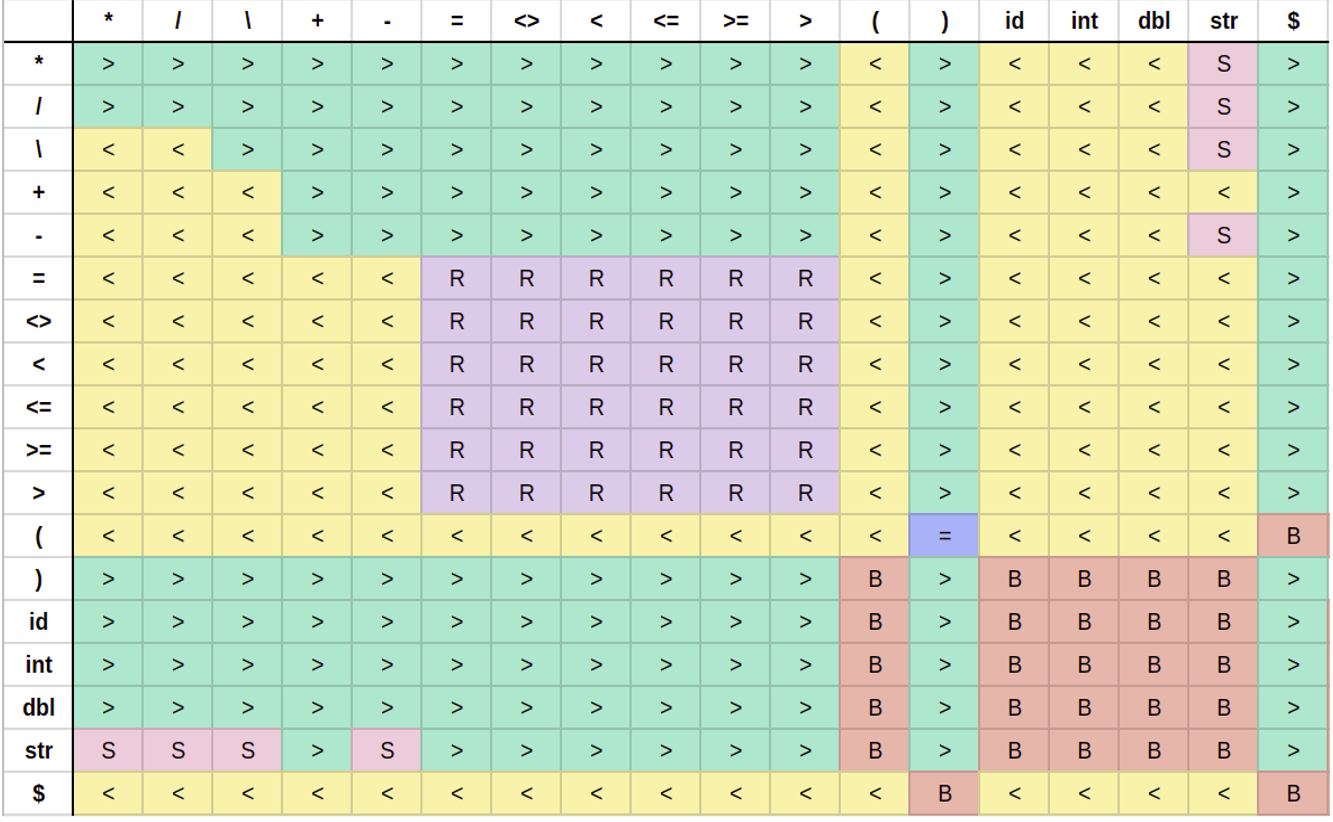
\includegraphics[width=15cm]{precTable.png}
                \caption{Precedenční tabulka}
                \label{obr:PT}
            \end{figure}

    \newpage



\section{Parser - Sémantika} \label{semantika}
    Implementoval xodehn08

    \subsection{Funkce}
    Sémantická analýza ověřuje sémantickou správnost zpracovávaného zdrojového kódu. V našem projektu je výstupem sémantické analýzy (tedy i parseru) Abstraktní syntaktický strom (AST), který je vstupem do generátoru cílového kódu.

    \subsection{Postup Implementace}
    Během syntaktické analýzy (práce parseru), který simuluje konstrukci derivačního stromu, probíhala i částečná sémantická analýza a zbytek u generování kódu. V parseru šli řešit sémantické akce typu: nedeklarované / nedefinované funkce a proměnné, špatný počet a datové typy parametrů funkcí, neslučitelné datové typy ve výrazech, atd. Těchto sémantických kontrol (akcí) lze dosáhnout použitím tabulky symbolů. V generátoru kódu se provádí např. implicitní konverze ve výrazech nebo kontrola dělení nulou.

    Implementace probíhala tak, že jakmile byl parser z větší části implementovaný, začal se do něj dopisovat kód pro provádění sémantických akcí.

    \subsection{Tabulka symbolů}
    Náš tým měl první variantu projektu. Tabulka symbolů se tedy implementovala jako binární vyhledávací strom. Do této tabulky symbolů si ukládáme vše, co potřebujeme např. jestli je uzel stromu proměnná nebo funkce, dále definice / deklarace proměnných a funkcí. U funkcí si dále ukládáme počet a datové typy parametrů a návratové hodnoty. U každé funkce si vytváříme \uv{menší} tabulku symbolů, do které se ukládají lokální proměnné (i parametry dané funkce).

    Do tabulky symbolů si neukládáme vestavěné funkce, které jsou implementované v generátoru kódu. Informace o nich jsou uloženy v samostatném poli, které se využije při kontrole volání funkce.

    \subsection{Abstraktní syntaktický strom}
    Součástí sémantiky je i vytvoření abstraktního syntaktického stromu (dále jen AST). Stejně jako sémantické akce i naplňování AST probíhá zároveň s prací parseru.

    AST je reprezentováno jako globální pole, které se postupně naplňuje uzly AST reprezentující příkazy. Příkazy a výrazy jsou reprezentovány dvěma strukturami. Přesný typ výrazu / příkazu je určen \uv{tagem} a \uv{op}. \uv{Op} je prvek typu union, který obsahuje struktury reprezentující konkrétní příkaz / výraz. Pro určení, se kterou strukturou z prvku "op" se pracuje, slouží prvek \uv{tag}, který je typu enum. Uzel AST pro výraz navíc obsahuje prvek \uv{datatype} určující datový typ daného uzlu (výrazu). \cite{AST:AST_in_C}

	\newpage


\section{Generátor}
    Implementoval xsopfp00

    \subsection{Generování cílového jazyka IFJcode17}
    Dojde-li program až ke generátoru, tak je vstupní program validní a dojde ke generování cílového jazyku IFJcode17. Generování probíhá vypisováním jednotlivých instrukcí jazyka IFJcode17 na standardní výstup. Na začátku generování je vždy vypsán úvodní řádek ".IFJcode17", který značí, že se jedná o jazyk IFJcode17 a následuje řádek obsahující instrukci se skokem na návěští hlavního bloku kódu (scope). Jelikož můžou následovat definice funkcí, tak je jako aktuální rámce nastaven lokální (LF).


    Poté začne generátor procházet AST, to je tvořeno polem ve kterém jsou seřazeny jednotlivé příkazy za sebou. Jakmile narazí generátor na prvek, který značí začátek hlavního bloku kódu tak pro něj vytvoří návěští a změní aktuální rámec na globální (GF). Generování jednotlivých prvků v AST je pak závislé na jejich typu (viz níže).

    Kvůli implicitním konverzím dochází u všech výrazů ke kontrole datových typů a k případné datové konverzi. To vše probíhá generováním potřebných instrukcí jazyka IFJcode17.

    \subsubsection{Generování funkcí}
    Hned na začátku definice funkce se pro funkci vygeneruje unikátní návěští. Po vytvoření návěští následuje přesun dočasného rámce na zásobník a proběhne nastavení návratové hodnoty funkce na implicitní hodnotu dle návratového typu funkce. Následuje generování bloku kódu uvnitř funkce a samotná funkce je následně ukončena přesunem aktuálního rámce do dočasného.

    \subsubsection{Generování vstupu od uživatele}
    Pokud dojde na generování vstupu od uživatele (Input), pak je nejprve vypsána hodnota "? ". Následuje instrukce READ, která obstará vstupní honotu a umístí ji do požadovaného rámce.

    \subsubsection{Generování podmínek}
    Každá podmínka nese informace o daném výrazu, bloku kódu uvnitř podmínky a ukazatele na další podmínku. Jelikož jsme implementovali i rozšíření IFTHEN, tak může první podmínka odkazovat na další (If-Then nebo else), nebo se může jednat pouze o jednu podmínku.

    Na začátku každé podmínky se nejprve vygenerují instrukce pro vyhodnocení daného výrazu. Je-li podmínka splněna, pak se vygeneruje daný blok kódu a na konci následuje skok na návěští, které je umístěno za všemi podmínkami. Pokud podmínka však splněna není, pak je proveden skok na následující podmínku (if-then nebo else).

    \subsubsection{Generování cyklů}
    Nejprve je vytvořeno unikátní návěští a následuje vytvoření nového dočasného rámce. Poté se vygeneruje výraz podmínky cyklu. Je-li podmínka splněna, dojde k vygenerování bloku kódu uvnitř cyklu a následuje skok na začátek cyklu. Pokud podmínka není splněna, pak následuje skok na konec cyklu.

    \subsubsection{Generování výrazů}
    Pro každou část výrazu se vytvoří nová proměnná, do které je umístěna hodnota daného výrazu. V průběhu toho dochází ke kontrole datových typů a k případným implicitním konverzím.
    Jedná-li se o pravdivostní výraz, pak následuje vytvoření potřebných skoků. Pokud se o pravdivostní výraz nejedná, je výsledná hodnota celého výrazu uložena do potřebné proměnné.

    \newpage

\section{Závěr}

    \newpage
    \bibliography{dokumentace}

\end{document}